\documentclass{sig-alternate}
\pdfpagewidth=8.5in
\pdfpageheight=11in
\usepackage{listings}
\lstset{language=Python}
\usepackage{color}
\usepackage{xspace}
\usepackage{url,moreverb,graphicx}
\usepackage{ifthen}
\usepackage{paralist}
\usepackage{lipsum}
\usepackage{tikz}
\usetikzlibrary{patterns}
\usepackage{pgfplots}

\clubpenalty=10000
\widowpenalty = 10000

\definecolor{lightgray}{rgb}{.9,.9,.9}
\definecolor{darkgray}{rgb}{.4,.4,.4}
\definecolor{purple}{rgb}{0.65, 0.12, 0.82}
\lstdefinelanguage{JavaScript}{
  keywords={typeof, new, true, false, catch, function, return, null, catch, switch, var, if, in, while, do, else, case, break},
  keywordstyle=\color{blue}\bfseries,
  ndkeywords={class, export, boolean, throw, implements, import, this},
  ndkeywordstyle=\color{darkgray}\bfseries,
  identifierstyle=\color{black},
  sensitive=false,
  comment=[l]{//},
  morecomment=[s]{/*}{*/},
  commentstyle=\color{purple}\ttfamily,
  stringstyle=\color{red}\ttfamily,
  morestring=[b]',
  morestring=[b]"
}

\lstset{
   language=JavaScript,
   backgroundcolor=\color{lightgray},
   extendedchars=true,
   basicstyle=\footnotesize\ttfamily,
   showstringspaces=false,
   showspaces=false,
   numbers=left,
   numberstyle=\footnotesize,
   numbersep=9pt,
   tabsize=2,
   breaklines=true,
   showtabs=false,
   captionpos=b,
   xleftmargin=4.0ex
}

\newcommand{\tool}{\textsc{ConcolicDOM}\xspace}
\newcommand{\code}[1]{{\texttt{#1}}}
\newcommand{\header}[1]{\par\smallskip\noindent\textbf{#1}}

\newboolean{showcomments}
\setboolean{showcomments}{true}
\ifthenelse{\boolean{showcomments}}
{\newcommand{\nb}[2]{
\fbox{\bfseries\sffamily\scriptsize#1}
{\sf\small$\blacktriangleright$\textit{#2}$\blacktriangleleft$}
}
}
{\newcommand{\nb}[2]{}
}
\newcommand\james[1]{\nb{James}{#1}}
\newcommand\eric[1]{\nb{Eric}{#1}}
\newcommand\ali[1]{\nb{Ali}{#1}}

\renewcommand*{\lstlistingname}{Sample Code}

\begin{document}

% --- Author Metadata here ---
\conferenceinfo{ISSTA 2014, Jul 21-26, 2014}{San Jose, California}
%\CopyrightYear{2014} % Allows default copyright year (20XX) to be over-ridden - IF NEED BE.
%\crdata{0-12345-67-8/90/01}  % Allows default copyright data (0-89791-88-6/97/05) to be over-ridden - IF NEED BE.
% --- End of Author Metadata ---


\title{{\ttlit ConcolicDOM:} Generating HTML for concolic testing JavaScript Web applications}
\numberofauthors{3} 
\author{
\alignauthor
James Lo\\	
       \affaddr{Department of Computer Science}\\
       \affaddr{University of British Columbia}\\	   
       \affaddr{Vancouver, Canada}\\
       \email{tklo@cs.ubc.ca}
\alignauthor
Eric Wohlstadter\\
       \affaddr{Department of Computer Science}\\
       \affaddr{University of British Columbia}\\	   
       \affaddr{Vancouver, Canada}\\
       \email{wohlstad@cs.ubc.ca}
\alignauthor
Ali Mesbah\\
       \affaddr{Department of Electrical and Computer Engineering}\\
       \affaddr{University of British Columbia}\\	   
       \affaddr{Vancouver, Canada}\\
       \email{amesbah@ece.ubc.ca}
}
\date{24 January 2014}

\maketitle
\begin{abstract}
\end{abstract}

% A category with only the three required fields
\category{D.2.5}{Software Engineering}{Testing and Debugging}[Symbolic execution, Test coverage of code, Test execution]
%A category including the fourth, optional field follows...
\category{D.3.2}{Software}{Programming Languages}[JavaScript]

\keywords{JavaScript, test runnability, HTML, DOM}

\section{Introduction}

JavaScript is increasingly a popular language for software implementation: %; and the World Wide Web is increasingly an attractive platform for delivering applications.
HTML5 and its standardization enable Web apps to have an interactivity and feature-richness comparable to those implemented for traditional desktops.  The latest round of browser wars makes executing JavaScript more efficient, robust, secure and consistent across platforms.  Because of HTML5, more desktop and mobile operating systems actually now support implementing native apps using the combination of JavaScript, HTML and CSS~\cite{jalangi}.
The Bring Your Own Device (BYOD) movement in Enterprise IT increases hardware heterogeneity, which also makes JavaScript apps\footnote{JavaScript apps are preferred in Web browsers because they are lighter weight than Java applets and they don't require installation of any proprietary plugins such as Flash and Silverlight} a convenient solution for delivering the application front end (e.g.~\cite{BNSFoffice365}).
Emergence of Node.js and its scalability also make JavaScript widely adopted on the server side.
Consequently, many institutions such as the Khan Academy~\cite{khanAcademy} use JavaScript for teaching programming; and JavaScript has consistently been a top 2 in the RedMonk~\cite{redmonk} popularity rankings.%~\footnote{results are based on projects hosted at GitHub and questions asked at StackOverflow}.

Yet, despite the language's ubiquity, testing JavaScript can be challenging and cumbersome.
For example, in a typical Web app, a lot of JavaScript code is intermixed with back end logic and front end HTML~\cite{QUnitIntro}.
Such intermixes introduce dependencies when trying to run JavaScript code, and test cases cannot be fully run until those dependencies are properly resolved.

In this paper, we elaborate on the HTML problem and present our approach to it.
In a Web app, HTML describes the graphical user interface, and JavaScript code that operate an API called the Document Object Model (DOM) are abundant, because the DOM API is the standard for accessing and mutating HTML.
When JavaScript code runs, its runtime execution would encounter DOM operations that would subtly imply the DOM having a particular tree structure. 
In other words, when trying to run a test case, if the DOM structure does not satisfy what the code expects it to be, execution would fail and the test case would terminate prematurely.
A recent study in the literature~\cite{frolin2013} discovered that the majority of bugs in JavaScript are related to operations on the DOM.

To further illustrate the necessity of a satisfiable DOM structure, suppose the function {\tt checkRows} in Sample Code ~\ref{dom0} is being unit tested concolic-ly.  
The function is simplified from a feature Chrome Experiment~\cite{domtris} that uses the DOM to implement Tetris.  
Concolic testing~\cite{cute} executes the app in a way to maximize path coverage; to do so, we must visit both the {\tt True} and {\tt False} branches of each {\tt if} statement in Sample Code ~\ref{dom0}.
\begin{figure}
\begin{lstlisting}[caption=Example that needs tracing and solver. The function getElementById() is equivalent to document.getElementById(),label=dom0]
function checkRows() {
  var field = getElementById("tetris"); 
  var i, row;
  for (i=field.children.length; i--;) {
    row = getElementById("row"+i);
    if (row.children.length === 10) {
      // ... row filled, update score
    }
  }
}
\end{lstlisting}
\end{figure}

To make the {\tt if} statement go to the {\tt True} branch, the web page's DOM structure must satisfy the following constraints:
\begin {compactitem}
\item there is an element with id {\tt tetris}
\item {\tt tetris} contains children elements, because we must first enter the {\tt for} loop
\item there are rows having id's the nomenclature {\tt row0}, {\tt row1}...
\item the number of rows must be greater than or equal to the number of children that {\tt tetris} has
\item at least one of the rows must have exactly 10 children
\end {compactitem}

While manual generation of HTML is possible, the manual approach would quickly become tedious and not scalable.  
The reason is that an unique DOM structure is required for going through different execution paths.  
For example, to go to the {\tt False} branch of the above {\tt if} statement, rows cannot have 10 children.
Therefore, when an {\tt if} statement depends on DOM operations to decide which branch to go, any addition of such {\\tt if} statements to the code would double the number of unique DOM structures for achieving path coverage, leading to exponential growth.
Moreover, because not every {\tt if} statement depends on DOM operations, manual generation can become complex and labour intensive to keep track of all relevant {\tt if} statements and multiple DOM elements involved.



% the problem can be hard
% manual generation
% random generation
% greedy or just in time generation ~\cite{ZenCoding}
% constraint-based generation
% constraint solver
% justify for tracing, look ahead, and generating constraints
% justify for using a solver, rather than heuristics to resolve constraints

% cannot generate HTML for game, 
Note that the code does not imply the following, which we take for granted in a Tetris game.
\begin {compactitem}
\item Each {\tt row} is a child element of {\tt tetris}.
\item Each {\tt row} is vertically stacked: {\tt row10} is right above {\tt row9}, which is also right on top of {\tt row8}, and so on.
\item Children of a {\tt row} are blocks that make up a piece.  
\item etc.
\end {compactitem}

manual generation
random generation


%contributions

0) DOM-specific tracing
1) DOM solver
2) Generating HTML
3) Integration with QUnit



DOM mutations
Attributes


Random testing, concolic testing... many prior work focus on generating inputs. 
However, the problem is that just having the inputs to a function is not sufficient.  
For example, DOMtris is a very simple Web implementation of Tetris, almost all functions don't have any input arguments.  
Yet, all these functions both depend on and mutate the state of the app.  
In the case of DOMtris, an example use case is to increase score and clean up the game pieces when the gamer has fully filled one or more rows.  
The DOM makes up a big part of a Web's app state.  
Thus in this paper we focus on the DOM.  
Indeed, DOM operations make up a majority of an app's execution and defects, according to a study by Frolin.  

A naive approach is to do just in time generation of the DOM.  
For example, if the statement is document.getElementById(), we can just return or create an element with "id".  
Yet there are 2 subtle issues.

First, there are multiple possible outputs.  

Second, dependencies in Wikipedia.  

Using a solver is easier and protects us from more complicated cases.

Our approach also supports concolic testing of DOM operations.



The new perspective is distinct from our previous motivation, which was using our tool to define test cases and drive run time execution of the program.  

Inputs can be defined for a test case in different ways: manually by test engineers writing test cases or automatically through concolic or random testing



\section{Challenges}
While trying to generate satisfiable DOM trees, we had to resolve the following challenges:  

\header{Single Clues are Incomplete.}  
% why tracing 
An intuitive approach would be to generate DOM elements "just in time"; however, such naive approach does not always work.  
Just in time generation is to greedily create whatever DOM elements necessary for satisfying the current single DOM operation.  
For example, in Sample Code \ref{dom0}, whenever {\tt getElementById()} is called, we could just create and return an ad-hoc DOM element having the corresponding id.  
When we see {\tt (row.children.length === 10)}, we could additionally create 10 ad-hoc children for the {\tt row}.  

The problem is that other DOM operations may contradict the ad-hoc DOM tree.  
A counter example we discovered very early is by just loading Wikipedia~\cite{wikipedia}.  
While loading the webpage, it executes the jQuery {\tt \$("\#B13\_120517\_dwrNode\_enYY")}, which is to get an element by a specific id.  
Then, some time later, the webpage calls {\tt \$("div\#B13\_120517\_dwrNode\_enYY")}, which is to get a <div> element by the exact same id.  
While the two jQueries may be written by different developers, we can easily see that the greedy approach does not work because it does not consider DOM operations in other parts of the code.
when trying to satisfy {\tt \$("\#B13\_120517\_dwrNode\_enYY")}, how do we know a <div> is the correct tag type to generate in the first place?  
If the generated DOM element is not a <div>, then the 2nd jQuery would return {\tt null}.  
There can be many different possibilities for satisfying a single current DOM operation; and picking the correct answer out of the many possible ones requires collectively tracing relevant DOM operations.  


\subsection{DOM Operations are Chained}
In JavaScript, a DOM operation of a DOM element (e.g. {\tt elem.parentElement}) usually returns another DOM element.  Thus DOM operations can be chained: {\tt elem.parentElement.parentElement}.  
Now consider we have multiple DOM operations.  What would the overall DOM tree look like?  How many children do {\tt b} and {\tt c} exactly have?  There are many possibilities, the search space of the solution is not small.    
\begin{compactitem}
\item {\tt elem.firstElementChild}: {\tt elem} has a first child.
\item {\tt b.lastElementChild}: {\tt b} has a last child.
\item {\tt b.parentElement}: {\tt b} has a parent.
\item {\tt elem.parentElement}: {\tt elem} has a parent.
\item {\tt elem.parentElement.parentElement}: {\tt elem} has a grandparent.
\item {\tt c.lastElementChild.previousSibling}: {\tt c} has a last child.
\item {\tt c.children[2]}: {\tt c} has 3 or more children.
\item {\tt b.nextElementSibling}: {\tt b} has a next sibling. 
\item ... etc.
\end{compactitem}

Because we need only one satisfiable DOM tree, it is possible to sort the DOM operations by element, and generate the DOM tree accordingly: 
\begin{compactitem}
\item {\tt elem.firstElementChild} 
\item {\tt elem.parentElement}
\item {\tt elem.parentElement.parentElement}
\end{compactitem}
\begin{compactitem}
\item {\tt b.lastElementChild}: {\tt b} has a last child.
\item {\tt b.parentElement}: {\tt b} has a parent.
\item {\tt b.nextElementSibling}: {\tt b} has a next sibling. 
\end{compactitem}
\begin{compactitem}
\item {\tt c.lastElementChild.previousSibling}: {\tt c} has a last child.
\item {\tt c.children[2]}: {\tt c} has at least 2 children.
\end{compactitem} 

\header{Indirect Influence.}  
% why backward slicing
While executing JavaScript code would subtly or passively imply the DOM having a particular tree structure (as in the jQuery example), sometimes the structure of the DOM tree would actively determine which branch a condition would go into.  
For example, in Sample Code~\ref{dom0}, we see that whether a {\tt row} has 10 children would actively determine whether the {\tt if} condition would go into the {\tt true} or {\tt false} branch.
While the DOM dependence is obvious in Sample Code~\ref{dom0}, very often DOM operations may not directly appear inside a condition: the result of different DOM operations may get assigned to multiple variables at various execution stages prior to the condition, either within the same function or up in the runtime stack.  
For example, a condition may appear as a simple {\tt if(a)} in the code; yet the variable {\tt a} can be {\tt (row.children.length === 10)} or something more complex, such as the result of multiple statements executed throughout the code.  
We have to backward slice variables so that we can accurately determine what DOM operations a condition may depend upon.  


\header{Dynamic Typing \& Dynamic Precedence.}  
% why dynamic analysis, not static analysis; why tracing and backward slicing both have to be dynamic.
JavaScript variables are dynamically typed.  Thus given a variable, we won't know exactly what type its value represents until we actually run the code.  
In our previous example, {\tt a} can be anything: an integer, a string, a boolean, or an object.  
Static analysis by itself is insufficient to detect which lines of code are DOM related.
Indeed, authors of existing JavaScript static techniques~\cite{staticJsWWW09, staticJsWWW11} reveal substantial gaps and false positives in their own work.  
Thus the only way to discover whether a condition contains DOM operations is to run the code.  Both tracing and backward slicing have to be dynamic to accurately determine which conditions depend on the DOM, and which don't.  

Dynamic precedence is another reason for conducting a dynamic backward slice.   
%What is the best and simplest way to incorporate dynamic tracing and dynamic backward slicing into the execution of JavaScript source code?  
%After all, if we were to support concolic testing, we must be able to accurately guide execution towards an intended path and thus we must properly understand how a condition would result in the {\tt True} and {\tt False} branches.    
%As stated in our contributions, our approach is generic, transparent, and browser independent; thus we cannot modify the source code of Web browsers and natively support slicing and tracing.  
%This is why we instrument JavaScript as it gets downloaded to the browser.  
% why decorated execution, not offline analysis 
%Adding to the overall complexity, conditions are usually composed of sub-conditions linked by logical operators (e.g. {\tt or}'s, {\tt and}'s, {\tt not}'s) nested inside one another.
%Executions of conditions can also have precedence.  For example, in an {\tt and}, when the first sub-condition is {\tt false}, the second sub-condition is never executed.  Similarly, an {\tt or} never executes the second sub-condition when the first returns {\tt true}.
% how is this a challenge
% drives the need for decorated execution, different from Jalangi

\begin{figure}
\begin{lstlisting}[caption=Example code showing DOM operations that are chained and conditions that have logical constraints interdependent with each other.  To make both of these {\tt if} statements true sub conditions i) and ii) become mutually exclusive: they cannot be true at the same time.  Thus a logic solver is required to generate a satisfiable DOM structure and HTML.,label=domOr]  
// ...
// Interdependent Logic Constraints
if (d === elem.firstElementChild // i)
 || d === b.lastElementChild) {}
// ... 
if (d === elem.parentElement // ii)
 || d === b.parentElement) {}
// ...

if (b.previousElementSibling === 
    c.firstElementChild) {}

// Chained DOM operations 
if (elem.parentElement.parentElement 
    === c.lastElementChild.previousElementSibling) {}  
if (c.children[2] === 
    b.nextElementSibling) {}  
}
\end{lstlisting}
\end{figure}

\header{Interdependent Logic.}  
% why solver, not heuristics 
Given a dynamic trace and a dynamic backward slice deduced from the logs of decorated execution, we would have a clear mapping between DOM operations and conditions; thus a logical approach would be to generate a DOM tree directly from the trace and backward slice.  
However, an heuristic approach may not always work because a condition may have logical constraints that are interdependent on logical constraints in other conditions.  
In an obvious example, 2 of the conditions in Sample Code~\ref{domOr}, the 2 {\tt if} statements, inter-depend on each other because of the DOM policy that a DOM element cannot be both a child and a parent of another DOM element.  
Specifically, sub-conditions {\tt i} and {\tt ii} must be mutually exclusive because {\tt d} cannot be both a child and parent of {\tt a}.
Therefore, when we want both of these {\tt if} conditions to be {\tt true}, a DOM specific solver is required to understand the unique policies of the DOM and make decisions accordingly for generating a proper satisfying HTML.

% \header{Implicit 2D Structure.}


\header{DOM Mutations.}  
% give update score as example
% why conditional slicing
% why 2D is more challenging than 1D
% why XML solver is not used 
Expressing the DOM for a solver is not as easy as expressing single dimensional numerical or string operations (e.g. additions and subtractions), because no solver supports 2D tree structures natively and DOM operations are more diverse.  
Mutations to the DOM tree structure must also be accounted for in both the backward slicing and the solver because changes to the HTML can happen any time during execution.  
Example mutations include adding or deleting a DOM element (e.g. in the use case of refreshing an email Inbox or deleting a message), or modifying the content or attributes within a DOM element.  

\section{DOM Constraints}
Given a piece of JavaScript code, along with the execution path that we intend the code to go into, 
our goal is to generate HTML so that the HTML would yield a DOM tree structure that would guide and support the execution of the code being tested.  

As an overview, our approach is to first instrument the JavaScript code so that we can log the code's execution for producing a dynamic backward slice and a dynamic trace.  
Next we analyze the trace and the slice to extract DOM-specific operations and to deduce constraints, which the DOM solver would take as input for generating a suitable DOM structure and corresponding HTML.  
Then we integrate the HTML into a test framework for running and asserting test cases.  

\begin{figure}
\begin{lstlisting}[caption=Example showing how code is instrumented for dynamic analysis.  The comment at line 9 shows the decorated object {\tt a} and its nested tree data structure.  
{\tt a}'s actual value is {\tt true} because both left and right hand side have the same value 10: {\tt line 11} and {\tt line 12},label=sheq]  
// Before Instrumentation
var row = getElementById("row"+i);
var a = row.children.length === b; 
if (a) {}

// After Instrumentation(i)
var row = _CALL(getElementById, _ADD(_CONST("STRING filename.js 0", "row"), i));
var a = _SHEQ(_GET(_GET(row, "children"), "length"), b);
/* a = {val: true
      , op:	_SHEQ
      , 0:	{val: 10, op:_GET, ...}
      , 1:	{val: 10, ...}}; */
if (__cond("IF_NAME filename.js 1", a)){}
\end{lstlisting}
\end{figure}

\header{Decorated Execution.}
Decorated execution is where we instrument the JavaScript code so that the execution of each JavaScript operator can be captured and decorated with additional data for producing a dynamic trace and a dynamic backward slice.  
Sample code \ref{sheq} illustrates the semantics of decorated execution.  
A general rule of thumb is that we transform each use of a JavaScript operator (e.g. {\tt .}) into a call to a corresponding operator function (e.g. {\tt \_GET()}).  
For example, {\tt row.children} becomes {\tt \_GET(row, "children")}.  {\tt \_SHEQ} represents the strict equal operator ({\tt ===}).  
Each operator function wraps (thus decorates) the actual computed value inside a decorated object that also contains data for tracing and slicing.   

A special case happens when we transform the {\tt \&\&} and {\tt |}{\tt |} ({\tt or}) operators, in which we have to consider the precedence of the operator's left hand side.   
For example, if the code is ({\tt a \&\& a.b}), the transformed version becomes {\tt \_AND(a, a.b)}; yet we do not want to execute {\tt a.b} when {\tt a} is {\tt null} or {\tt undefined}.  
A possible solution is to reuse {\tt a}: {\tt \_AND(a, a \&\& \_GET(a, "b")}.  
However, the left hand side can be a call to a function that may change the internal state of the application: e.g. {\tt appendLog() \&\& update()}.
Thus our solution is to assign the left hand side into a temporary variable, and then check the value of the temporary variable before executing the right hand side: 
{\tt \_AND(t = a, t \&\& \_GET(a, "b"))} and {\tt \_AND(t = \_CALL(appendLog), t \&\& \_CALL(update))}.  

Another special case is the {\tt ++} and {\tt ---} operators.  
For example, with {\tt i++} we have to first assign the original value of {\tt i} to a temporary variable before incrementing {\tt i}, then we return the temporary variable.
% functions, boundary to native functions


\header{Backward Slicer \& Post Order Traversal.}
% would a diagram be good?
The data structure of the decorated objects can be seen as a nested or tree structure because the calls to the operator functions are nested inside one another.  
For example, in Sample Code \ref{sheq}, the call to {\tt \_GET(..., "length")} is nested inside the call to {\tt \_SHEQ()}.  
Therefore, if we simply put the name of the operator function (e.g. {\tt "\_GET"}, {\tt "\_SHEQ"}, ...), inside the trace data, we can easily generate a backward slice via a tree traversal.  

In Sample Code \ref{sheq}, the variable {\tt a} equals to ({\tt row.children.length === b}).  
Thus {\tt a}'s backward slice must contain the backward slice of {\tt b} and the backward slice of {\tt row.children.length}, linked by the strict equal ({\tt ===}) operator.  
At line 8, the decorated object returned by {\tt \_SHEQ()}, assigned to the variable {\tt a}, is the tree parent of 2 decorated objects: {\tt b}, and the decorated object returned by the {\tt \_GET()} call.  

The tree children of a decorated object always come from earlier executions, e.g. {\tt \_GET(..., "children")} is executed before {\tt \_GET(..., "length")} before {\tt \_SHEQ(..., b)}.
Thus the tree's hierarchical structure is reversely proportional to the temporal order in which the operator functions are executed.  

During the traversal, we identify conditions that contain DOM operations and extract these DOM operations accordingly.  
In a chain of DOM operations, the operations closer to the chain head always come from earlier executions, thus the tree's hierarchy is also reversely proportional to the chaining order of DOM operations.  
The backward slicer traverses the decorated objects in post order, which is bottom up from leaf to root.  
This way, the dynamic backward slice not only yields a temporal history of the code's runtime execution, it also conveniently traces the DOM operation chains in the order from head to tail.

Each tree leaf represents an input or a constant.  
For example, a dynamic backward slice of {\tt row} would lead us to the DOM element with ID {\tt "row"+i}, where {\tt "row"} is a constant string, 
and {\tt i} has a backward slice leading to {\tt field.children.length}, which would lead us to the DOM element with ID {\tt "field"}.  
Because variables can be used multiple times, each variable can belong to more than 1 tree and can have more than 1 parent.  
Thus the data structure would appear more like a directed acyclic graph than a tree, even though a variable would never be a tree ancestor of any of its own ancestors.  

\begin{figure}
\begin{lstlisting}[caption=DOM constraints for generating an HTML that would satisfy for going the {\tt True} branch in the {\tt if} statement of Sample Code ~\ref{dom0}.  The constraints are shown in the input format for the CVC~\cite{cvc3} implementation of the SMT solver. {\tt \%} is the comment operator in CVC.,label=constraints0]
% document.getElementById("field");
% document.getElementById("row"+0);
ASSERT DISTINCT(field, row0);

% (field.children.length)--;
ASSERT childrenLength(field) > 0;

% row.children.length === 10;
ASSERT childrenLength(row0) = 10;
\end{lstlisting}
\end{figure}

\header {Trace Mapper \& Constraints Deducer.} 
For each instance that a condition is executed, the backward slicer would yield what DOM operations the instance has and how these DOM operations are related or interdependent on one another.  
Because each condition can get executed more than once at different time points, the MapDeducer would aggregate all executed conditions, map them according to their ID, and deduce constraints for the DOM solver to generate a satisfiable HTML.  
The MapDeducer works like MapReduce~\cite{mapreduce}.  So far everything is code-oriented in which we focus on each condition and its dynamic backward slice.  The MapDeducer would transition the focus to be DOM-oriented in which we assemble clues about the same part of the DOM tree that are scattered across multiple lines of code.  
The MapDeducer would put together the processed clues across multiple parts of the DOM tree back together, into a single set of constraints for the DOM solver to generate a satisfiable HTML.

Sample Code~\ref{constraints0} illustrates constraints for going to the {\tt true} branch of the {\tt if} statement in Sample Code~\ref{dom0}, resulting in Sample Code ~\ref{html0}.  
If we want to go to the {\tt false} branch, e.g. {\tt ASSERT NOT(childrenLength(row0) = 10)}, then the solver would generate a number of children not equal to 10 for {\tt row0}.  The exact number of children has not been deterministic based on our experiments: sometimes {\tt row0} has 2 children, sometimes {\tt row0} has none.  
%Recall the jQuery example from the Challenges section.  The MapDeducer would 

\begin{figure}
\begin{lstlisting}[caption=Example HTML generated by the DOM solver based on the constraints defined in Sample Code ~\ref{constraints0}.  Note that {\tt row0} is not a child of {\tt field} because the source code in Sample Code \ref{dom0} did not require the rows to be children of {\tt field}.,label=html0]  
<span id="field"><span></span></span>
<span id="row0">
  <span></span><span></span>
  <span></span><span></span>
  <span></span><span></span>
  <span></span><span></span>
  <span></span><span></span>
</span>
\end{lstlisting}
\end{figure}

\section{DOM Solver}
The DOM solver takes the constraints defined by the MapDeducer and attempts to generate a satisfiable DOM structure.  The solver is implemented as an extension of a SMT solver~\cite{cvc3} and would report anything not satisfiable.  

\header{DOM Tree \& DOM Operations.}
A major part of the DOM is its single parent, multi-children tree structure.  When generating a satisfiable DOM, we use the execution of DOM operations to infer the overall DOM tree.    
Each DOM operation in any line of code is like a piece of a puzzle describing a subset clue of the overall DOM tree.   
For example {\tt a = elem.parentElement.nextElementSibling} implies 2 subset clues: {\tt elem} has a parent element, and the parent has a sibling.  
Note that if the condition is {\tt a = elem.parentElement.nextElementSibling === null}, then the clues become {\tt elem} has a parent element, yet the parent has no next sibling and thus is the last child.

That said, questions remain unanswered about exactly where does {\tt elem} fit in or belong in the overall DOM tree; and other DOM operations would provide clues for that.  The DOM solver would take all the clues and generate a satisfiable structure.   

\begin{figure}
\begin{lstlisting}[caption=HTML generated for guiding the execution to follow the {\tt true} branch in the {\tt if} statement in Sample Code\ref{dom0}.label=htmlExtended]  
<span id="c">
  <span/>
  <span id="b">
    <span id="d">
      <span id="elem"/>
    </span>
  </span>
  <span/>
</span>
\end{lstlisting}
\end{figure}


% XPath
% how to create rules in DOM solver, example rules.  Intuition behind it.
% why not XML solver, not scalable
% SMT-lib language, swappable between CVC and Z3.
	% take advantage of Moore's law in terms of hardware performance and breakthroughs in constraint solvers
	% future compatibility for multiple data types

\header{DOM Operations into SMT Quantifiers.}	
In the solver we transform each DOM operation into a SMT function.  We then use quantifiers (e.g. {\tt EXISTS}, {\tt FORALL}) to define how the SMT functions relate to each other.  
Sample Code ~\ref{childrenLength} shows the boolean functions and integer functions we defined for supporting the {\tt elem.children.length} operation.  We first quantify the parent-child relationship: 
\begin{compactitem}
\item a node cannot be a child of itself, see {\tt line 1} and {\tt line 4} in Sample Code ~\ref{childrenLength}.
\item a child of a node cannot be the node's parent at the same time: {\tt line 8}.
\item a child can have only 1 parent: {\tt line 13}.
\end{compactitem}
Next, we define how children are ordered and quantify {\tt children.length}:
\begin{compactitem} 
\item first child starts at position or index 0: {\tt line 18} and {\tt line 24}.
\item last child has the largest child index: {\tt line 30}.
\item {\tt children.length} equals to one plus the child index of the last child, because the first child starts at position 0: {\tt line 40}.
\end{compactitem}
The parent SMT functions are quantified as the inverse of the child SMT functions (e.g. {\tt line 48}).  Similar to {\tt firstChild()} and {\tt lastChild()}, the sibling SMT functions are defined by extending {\tt children(x, y, j)}.  
For example, the next sibling of a node has the same parent and child index {\tt j+1}, when the node has child index {\tt j}.

\begin{figure}
\begin{lstlisting}[caption=SMT functions for defining the children.length DOM operation.  We start with defining the parent-child relationships; then move on to the ordering of children; then use the child index of the last child to define and quantify the {\tt childrenLength()} boolean function,label=childrenLength]  
% child(x, y): x is a child of y.
child: (Node, Node) -> BOOLEAN;	

% x cannot be a child of itself.
ASSERT FORALL (x: Node):	
  NOT(child(x,x));
	
% when y is the parent of x,
% then y cannot be a child of x.  
ASSERT FORALL (x, y: Node):
  child(x,y) => NOT(child(y,x));
  
% a child has only 1 parent.
ASSERT FORALL (x, y, z: Node):
  (child(x,y) AND DISTINCT(y,z)) 
    => NOT(child(x,z));

% x is the j-th child of y.
children: (Node, Node, INT) -> BOOLEAN;
ASSERT FORALL (x,y:Node, j:INT): 
  children(x, y, j) => 
    child(x, y) AND j >= 0;

% child position/index starts at 0.
firstChild:		(Node, Node) -> BOOLEAN;
ASSERT FORALL (x, y:Node):
  firstChild(x, y) <=> 
    children(x, y, 0);

% every other child must have an index 
% smaller than that of the last child.
lastChild: (Node, Node) -> BOOLEAN;	
ASSERT FORALL (x, y:Node): 	
	lastChild(x, y) => EXISTS(j:INT): 
	  children(x, y, j) AND 
	  (FORCALL(z:Node, k:INT): 
	    (children(z, y, k) AND 
	    DISTINCT(z, x)) => k < j);

% children.length equals to the
% child index of the last child.
childrenLength:	(Node) -> INT;
ASSERT FORALL (y:Node, j:INT):
	childrenLength(y) = j <=> 
	  EXISTS(x:Node): (lastChild(x, y) 
	    AND children(x, y, j-1));

% example of inversion
% y is the parent of x, is the same as 
% x is a child of y.
parent: (Node, Node) -> BOOLEAN; 
ASSERT FORALL (x, y: Node): 
  parent(y, x) <=> child(y, x); 
\end{lstlisting} 
\end{figure}

\header{Negation.}
We use the CVC implementation of SMT, which natively supports booleans and integers by default.  
%While it is possible to define a customized data structure to mimic the DOM tree in CVC, the boolean/integer function approach is simple and convenient for negating conditions and going into different execution paths.
%Because Web browsers also support accessing the DOM tree via XPath~\cite{documentEvaluate}, we defined additional SMT functions: {\tt following\_sibling}, {\tt preceding\_sibling}, {\tt descendant} and {\tt ancestor}.

\header{Solver Output into HTML.}
Because we used Boolean functions and Integer functions, CVC is only going to solve for the interdependent logic constraints and it does not directly yield a concrete DOM tree.  
Instead, CVC only expands the quantifiers and it outputs more {\tt ASSERT} statements for making the constraints satisfiable.  

In Sample Code \ref{domOr}, the condition inside the first {\tt if} statement has 2 sub conditions: 
\begin{compactitem}
\item {\tt d===elem.firstElementChild} ({\tt line 3}), and 
\item {\tt d===b.lastElementChild} ({\tt line 4}).
\end{compactitem}
When the DOM solver solves this {\tt if} statement for going to the {\tt true} branch, it would output {\tt "ASSERT lastChild(d, b);"} because it has decided on making the second sub condition ({\tt line 4}) {\tt true}.

To build the DOM tree, we built an API that parses the CVC output and builds a model for the DOM.  
In the CVC output, CVC creates many temporary variable names, thus each DOM element can have more than one alias.  
To consolidate the aliases, we start with DOM operations expressing the parent child relationship because each child can have only 1 parent.  
We also used other deterministic DOM operations such as {\tt firstChild()} and {\tt lastChild()} to group aliases together.  
For example, if {\tt x} is the first child of {\tt y} and {\tt z} is also the first child of {\tt y}, then {\tt x} and {\tt z} are two aliases of the same DOM element.  

Once the parent child relationship is established, our next step is to organize the ordering of children.  
Some DOM children have their positions explicit (e.g. {\tt firstChild(x, y)}, {\tt lastChild(x, y)} and {\tt children(x, y, j)}), yet very often the child parent relationship is implied.  For example, {\tt nextSibling(x, z)} implies {\tt x} and {\tt z} share the same parent.  
To calculate the ordering of children, we use the explicitly positioned children as anchors and we relate the anchors to other children by the sibling operations.  

%In case of any uncertainty, we would query the CVC model.  We have to do a binary search because querying the CVC model supports only {\tt true} or {\tt false} answers.  
%Because CVC does not support strings natively, for now we map tag names into integers in CVC.  <span> is the default tag type because <span> is an inline element and not a block.
%Once the DOM tree is defined, we search for the root of the DOM tree (the element without a parent) and generate HTML.  

% \header{DOM mutations.}

% \header{Conditional Slicing.}

\section{Implementation}
\label{impl}
\header{Concolic Driver.}
In the iterative process of concolic testing, we implemented a concolic driver that would repeatedly
\begin {enumerate}
\item Open the target URL
\item Load the generated html (initially empty html)
\item Execute the target JavaScript code
\item Measure coverage, and decide which path to go next
\item Call the MapDeducer, which returns the DOM constraints in text
\item Send the constraints to the DOM solver, which returns a satisfiable DOM tree
\item Go back to step 1 with the newly generated HTML.
\end{enumerate}
The concolic driver would iterate the cycle until it has reached a certain point, which can be configured to be a specific number of iterations (e.g. 1,000 DOM trees generated), a certain level of coverage (e.g. 100\% branch coverage), or both. 


\header{Instrumenting and Executing JavaScript.}  
Our approach has to be generic, transparent and browser-independent.  
We use Selenium's WebDriver\cite{webdriverjs} to drive Web browsers for executing JavaScript.  WebDriver runs on multiple browsers, including headless browsers such as PhantomJS~\cite{phantomjs}.  

When JavaScript is getting downloaded onto a Web browser, we use the WebScarab proxy to intercept the download and to instrumenting code.  
The proxy passes intercepted JavaScript code to the Google Closure Compiler API~\cite{ClosureCompiler} for transforming JavaScript into calls to the operator functions. 

Both the Backward Slicer and MapDeducer are implemented as JavaScript APIs, and WebDriver natively supports calling JavaScript functions within the browser.  
Thus our approach is entirely transparent and can be applied to multiple brands of Web browsers.    


\header{DOM Solver.}  
CVC allows writing the constraints in Java, yet we do not want to hardcode the constraints because the constraints are different in each execution path.  
Thus we use Java's ProcessBuilder~\cite{processbuilder} class to communicate with the executable (.exe) version of CVC.  We decided to use CVC3 rather than CVC4~\cite{cvc4} because CVC3 is generally more stable during our experimentation.  
The API that parses the CVC output is also implemented in Java, thus we used the W3C DOM API~\cite{DomAPI} for generating HTML.  
%QUnit provides a <div> called the fixture which can be set as the HTML for a test case.   Before execution, WebDriver would set the {\tt innerHTML} of the fixture element to the generated HTML.  


\header{Limited Path Coverage.}  
% zero, 1 and n.
Very often we would not know how many times to execute a loop.  For example, in Sampe Code ~\ref{dom0}, there is no upper limit to the number of children that {\tt field} can have.  
\tool would execute loops zero, one, and {\tt n} times, where {\tt n} can be configured for a particular loops or for all loops.  Thus \tool would achieve limited path coverage rather than full path coverage.  


\header{Indexing Functions.}  
Most of the time JavaScript functions are defined inside closures and are not accessible~\cite{privatefunctions}.  
When we instrument JavaScript code, we extract the functions by assigning them to an object that we have access to.  Because functions can have the same name, we use the node number in the JavaScript Abstract Syntax Tree as ID.


\header{{\tt eval()} \& inline JavaScript.}  
In addition to source files, JavaScript code can also be found within {\tt eval()} and inlined as attributes of a DOM element inside the HTML declaration (e.g. {\tt <body onload="runFunction()">}).
We instrument each {\tt eval(code)} statement into {\tt eval(instrument(code))}.  We cannot override the native {\tt eval()}, because the native {\tt eval()} must be called inside the closure to give {\tt code} access to the closure's local variables.  
The {\tt instrument()} function would send the {\tt code} to the proxy for instrumentation via a XMLHttpRequest.  

To instrument inline JavaScript, we traverse the original HTML using the JSoup API~\cite{jsoup}.  Once we detect DOM attributes that contain JavaScript, we pass the JavaScript to ClosureCompiler for instrumentation.  
For newly created elements, e.g. {\tt elem.innerHTML = text}, we use getters and setters to detect the new elements.  Once detected, we traverse the new elements, extract JavaScript and call the {\tt instrument()} function.  
% Tudu

%\header{QUnit}
%\tool has integration with QUnit~\cite{qunit} so that existing test suites can automatically take advantage of \tool without additional manual effort.  
% \tool is also extensible to be integrated with other test frameworks~\cite{jstests}.
% Thus given a test case, be its inputs were generated manually or automatically, \tool can be used to help the test case and its assertions get fully utilized.

\section{Evaluation}
Our evaluation would take the form of a case study in which we would compare different approaches to testing the {\tt function checkRows()} in Sample Code \ref{dom0}, and measure how much coverage each approach can achieve.
The 3 approaches being compared are:
\begin{compactitem}
\item {\em Without HTML}
\item {\em Existing HTML} from the application
\item \tool generated HTML
\end{compactitem}

For each approach, we would follow the same methodology of loading and execution the function:
\begin{compactitem}
\item Load the target URL
\item Load the HTML (except {\em Without HTML})
\item Execute the target code
\item Measure coverage
\end{compactitem}
Recalling from the Implementation section, the 4 steps above are identical to the initial 4 steps that our concolic driver would take in each iteration.  Additionally the concolic driver would take the executed paths as feedback and generate new HTML.  
For {\tt function checkRows()}, we can simply call the function via {\tt checkRows()} because it does not take any input arguments.

\begin{figure}
\centerline{\scalebox{0.38}{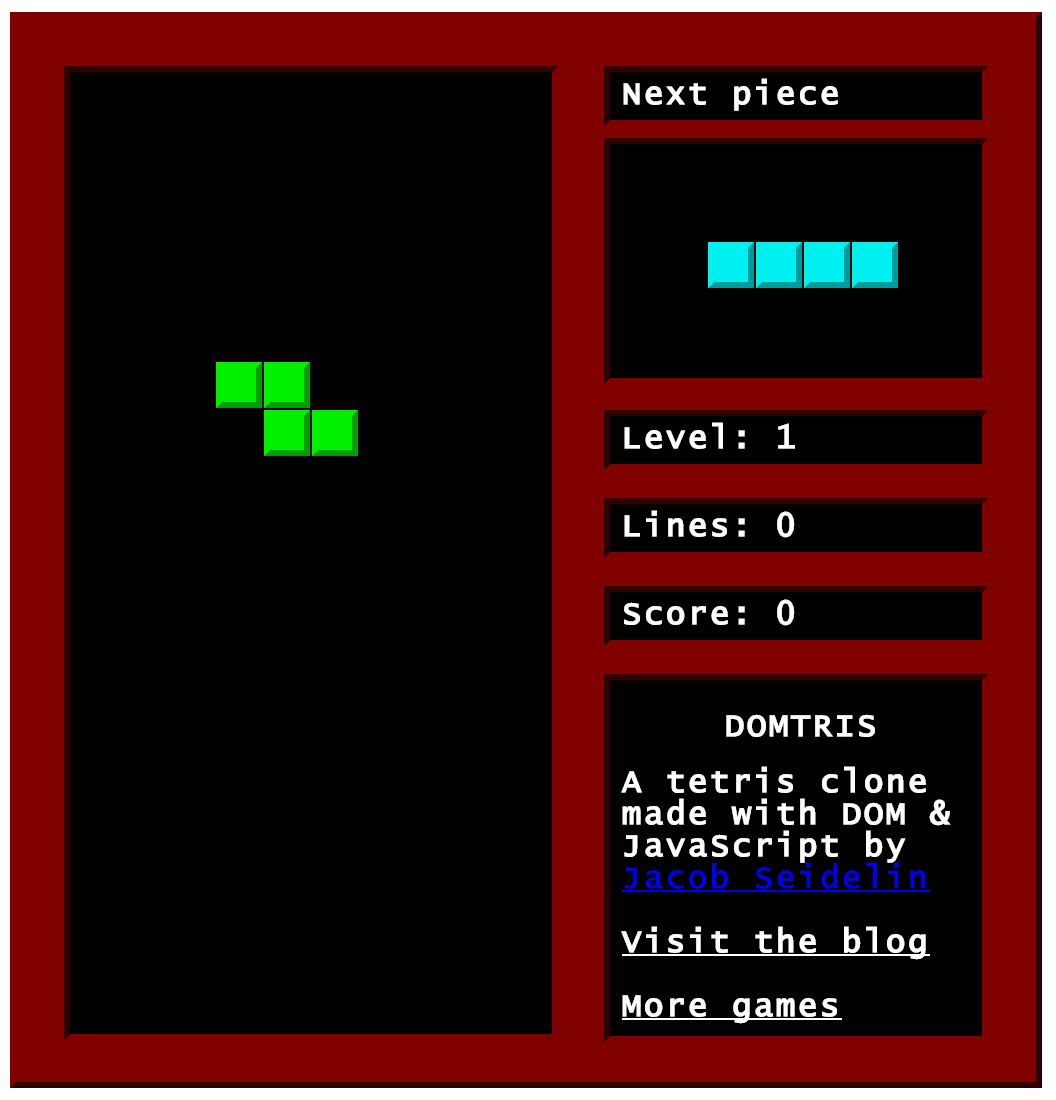
\includegraphics[natwidth=1056,natheight=1100]{domtris.png}}}
\caption[DOMtris game field]{The DOMtris game field has 20 rows, thus {\tt field.children.length} is set to be 20 in our evaluation.}
\label{domtrisfield}
\end{figure}

\begin{figure}[h]
\centerline{
\begin{tabular}{*2l|*3c}
\hline
& & \multicolumn{3}{c}{Count (Number Of)} \\ 
App & Function & Statements & Branches & Paths \\ \hline
DOMtris & checkRows() & 6 & 4 & 41 \\ \hline
\end{tabular}
}
\caption{Number of Statements, Branches and Paths of function being evaluated.}
\label{paths}
\end{figure}

\header{Counting Execution Paths.}
Figure \ref{paths} shows the number of statements, branches and paths that the function has.   
When counting the number of paths in the {\tt function checkRows()} in Sample Code \ref{dom0}, 
the original code does not pose an upper bound to the number of times the {\tt for} loop would get iterated because {\tt field.children.length} can be any value.
Therefore, we would set {\tt field.children.length} to a specific number for calculating the total number of possible execution paths in the function.
{\tt field} is set to have 20 children because the actual application always has 20 rows (Figure \ref{domtrisfield}). 
The following shows how the number of statements, branches and paths are counted for the {\tt function checkRows()}:
\begin{compactitem}
\item {\em Statements}: 6, {\tt line 2} to {\tt line 7}, inclusive.
\item {\em Branches}: 2 + 2. The {\tt for} loop has 2 branches: {\tt stay} and {\tt break}; plus the {\tt if} condition also has 2 branches: {\tt true} and {\tt false}. 
\item {\em Paths}: 20 ({\tt stay} branch in for loop) * 2 ({\tt true} and {\tt false} branches in {\tt if} statement) + 1 ({\tt break} branch).
\end{compactitem}

\begin{figure}[h]
\centerline{
\begin{tabular}{l|*3c}
\hline
& \multicolumn{3}{c}{Count (Number Of)} \\	
Approach & Statements & Branches & Paths \\ \hline
Optimal & 6 & 4 & 41 \\ \hline
{\em Without HTML} & 1 & 0 & 0 \\ 
{\em Existing HTML} & 5 & 3 & 1 \\ 
\tool & 6 & 4 & 41 \\ \hline
\end{tabular}
}
\caption{Statement, Branch and Path coverage of different approaches to testing the {\tt function checkRows()}. The Optimal approach is stated here to reference what perfect coverage would look like.}
\label{coverage}
\end{figure}

\header{Coverage Results.}
Figure \ref{coverage} shows the coverage results of different approaches to testing the {\tt function checkRows()}.  

The {\em Without HTML} approach cannot cover any statement because the first statement in the {\tt function checkRows()} is already a DOM operation requiring the existence of an element with {\tt id} {\tt "field"}.

The {\em Existing HTML} approach is able to cover 5 statements inclusively from {\tt line 2} to {\tt line 6} because the original HTML already has 20 rows inside {\tt field}.  
However the {\em Existing HTML} approach cannot cover the statement in {\tt line 7} because the rows do not have any children at the start of the game. 
{\em Existing HTML} is able to cover 3 of the 4 possible branches: both the {\tt stay} and {\tt break} branches in the {\tt for} loop, and the {\tt false} branch in the {\tt if} condition. 
Yet, the {\em Existing HTML} approach is able to cover only one path because going through a different path in {\tt function checkRows()} requires another unique DOM tree structure.  

\tool is able to cover all possible paths in {\tt function checkRows()} because we have set {\tt field.children.length} to be 20, 
and all the conditions (the {\tt for} loop and the {\tt if} condition) inside the function are all driven by DOM operations.  
In case when there are conditions that are driven by other data types, our solver would have to be extended to support these data types.    

\header{Discussion.}
In the specific example of {\tt function checkRows()}, using only the existing HTML is sufficient to achieve high statement coverage (5/6 or 83\%) and high branch coverage (3/4 or 75\%).  

Concolic testing often takes additional time, in our small example the DOM solver would take about 15 to 30 seconds to generate each additional HTML.
Thus whether concolic testing is worth it would depend on how much additional coverage the concolic approach would provide, and the benefits of having the additional coverage.  

While \tool covers only 1 additional statement ({\tt line 7}) and only 1 additional branch ({\tt true} branch of the {\tt if} condition) compared to {\em Existing HTML}, 
the additionally covered statement is responsible for updating the game's score, and scoring is a core functionality of DOMtris.  
Another benefit of \tool is that it covers all the different paths that generate the different permutations of increasing the score.  

Our current concolic driver is primitive in the sense that it exhaustively tries to cover all execution paths possible.  
In the future, it may be worth investigating if it is possible to design a smarter concolic driver that can give priority to execution paths that would yield the highest marginal benefit of additional coverage: 
e.g. highest additional branch coverage, the most diverse permutation of increasing the score, etc.  
That way the tester can exercise concolic testing partially, combine concolic testing with other less expensive testing methods, and still achieve certain desired outcomes without incurring the full costs associated with complete concolic execution.  
Thus having a prioritized concolic engine would give the tester greater control to manage the costs and benefits of the testing life cycle.  

% yahoo
% Tinysort
%  http://tinysort.sjeiti.com/
% Zen Coding
%  http://zen.sjeiti.com/
% DOMtris
%  http://www.ugrad.cs.ubc.ca/~k5r4/nbpAFZyrx5o/tracing/domtris/domtris.html
% Tudu
%  http://app.rasc.ch/tudu/welcome.action
% Knockout:
%  http://knockoutjs.com/examples/ 
% JQuery Widget: 
%  http://jqueryui.com/demos/
%  http://wijmo.com/widgets/
% Tizen
%   https://developer.tizen.org/downloads/sample-web-applications
%			mancala

\section{Future Work}
% element vs. node
% inheritance in CVC


Indeed, the majority of JavaScript bugs are DOM related~\cite{frolin2013}.
Ultimately, our higher level goal is to foster closer collaboration among designers and developers.\footnote{As part of separating concerns, design and development are often done by distinct individuals having very different backgrounds.}
For example, because \tool generates reference HTML for satisfying code execution, it can be used to detect DOM mismatches between the designer's HTML vs. what is expected in the developer's JavaScript code.
A mismatch may not always be the developer's fault.  Sometimes it is possible that the designer may have made a mistake when updating the HTML or may be just too busy and have forgotten to notify the developer about a change.

\section{Related Work}
%Whether the test inputs are manually, randomly (e.g. ~\cite{artemis}) or symbolically (e.g. ~\cite{kudzu, jalangi}) defined.


\header{Concolic Testing.}
% cute, jalangi, kudzu, eventConcolic
%Having the constraints generated from a backward slice, concolic testing would use a constraint solver to generate input that would eventually drive the execution of each condition towards a specific branch.  
While there have been numerous publications on concolic testing (e.g. ~\cite{cute, klee, eventConcolic}), 
Kudzu~\cite{kudzu} and Jalangi~\cite{jalangi} are the only two for concolic testing software that are written in a dynamically typed language; and both focus on JavaScript.  

A main contribution of Kudzu is a string solver that can handle select regular expressions.  
The solver is deployed to generate strings as UI inputs for detecting security vulnerabilities in JavaScript Web applications.   
A main contribution of \tool is our DOM solver.  Our solver generates HTML for running and testing JavaScript code that contains DOM operations.    
While DOM trees are usually represented in HTML string form, designing a DOM solver is different from designing a regex string solver.
As discussed in the Challenges section, the main reasons are that the DOM solver has to support a 2D hierarchical tree structure while strings are usually single dimensional.  
Moreover, inferring implicit clues from DOM operations is also different from inferring regex patterns.  
In addition, the architecture of \tool is implemented to run on multiple Web browsers, while Kudzu runs only on their single proprietary browser that supports Kudzu's component~\cite{flax} for tracing and slicing.    

A main contribution of Jalangi is their system of shadow values for selective record and replay.  
In the shadow system, they encapsulate each data value into an object; the encapsulated object can contain any metadata (the shadow) about the actual data value.  
While our system of decorated execution is similar to Jalangi's shadow system, a tester using Jalangi would manually identify which variables are inputs and would manually specify each input's type.  
Jalangi then generates various input values for those variables that are manually identified by the tester.  
In contrast, \tool uses post-order tree traversal for automatically identifying possible inputs.  

When \tool instruments JavaScript, it would label each constant value as a constant.
For example, the JavaScript statement {\tt var x = "string";} would be instrumented into {\tt var x = \_CONST("string");}.  
  
Therefore, during the post order traversal, if a tree leaf of the decorated objects tree is not labelled, the variable inside the leaf would be identified as a candidate input, 
because the data value does not come from within the code.  
\tool generates a dynamic backward slice and thus executes the code, therefore the data type of candidate inputs can easily be determined from the actual data value.  

Another differentiation is that for supporting the DOM we designed a Trace MapDeducer for extracting and transforming code-centric backward slice into DOM-centric constraints for the DOM solver.  
Both CUTE~\cite{cute} and Jalangi use the CVC3~\cite{cvc3} solver for supporting integers and strings.  

%jalangi and Kudzu focuses on generating inputs, and did not address the problems of closures and making test cases runnable.
% Whether these test cases are generated manually, randomly (e.g. ~\cite{artemis}) or symbolically (e.g. ~\cite{kudzu, jalangi}), these test cases cannot be properly run or asserted because 


% may move to Intro
%\header{HTML Generation.}
%\header{Emmet or Zen coding.}
%Emmet (formerly Zen coding) \cite{ZenSjeiti, ZenCoding} generates DOM elements as output.  
%Input to Emmet is the abbreviation of a CSS query that precisely specifies the DOM structure in a declarative manner.
%A major difference is that \tool solves for complex logic constraints (e.g. AND, OR conditions).
%Pythia uses the Web app's existing HTML.


\header{Constraint Solvers.} 
% xml solver, cvc, z3
Constraint solvers (e.g. SAT solvers) solve for parameters that satisfy a set of predefined constraints.  

Genev\`{e}s et al. developed an XML solver~\cite{xmlsolver} that takes limited XPaths as inputs; then it outputs XML that would satisfy those XPath conditions. 
Initially we intended to extending the XML solver.  However, after experimentations, we find it difficult to encode DOM node attributes into the XML solver and 
more importantly the XML solver is not scalable to more than 5 unique nodes. 

CVC~\cite{cvc3, cvc4} is a general purpose SMT solver and it is more scalable.  
However, being a general purpose solver also means that CVC does not natively support the tree structure defined in the DOM API.  
Our DOM solver uses quantifiers to encode and model the DOM within CVC.  
Nevertheless, the output of CVC yields only a description of the desired DOM tree (e.g. node A is child of node B), rather than the actual XML/HTML. 
Thus we have to take additional steps to transform CVC outputs into HTML.


\header{Feedback Directed Testing.}   
Feedback Directed Testing is an adaptive testing approach that uses the outcome of executing an input, to determine what the next input should be for achieving a goal, mostly maximizing coverage.  
Random testing and concolic testing are two major formats of feedback directed testing that is automated.  
Concolic testing is a form of feedback directed testing because it conducts backward slicing to generate inputs, and then it uses the resulting executed path as feedback for generating new inputs.  

In random testing for JavaScript Web applications, Artemis~\cite{artemis} randomly generates initial inputs and uses the output of functions (rather than executed paths) as feedback, for increasing coverage.  
Pythia~\cite{pythia} also generates initial inputs randomly, their feedback is changes to a state flow graph model, and their goal is to maximize the number of functions being called.  
The number of functions being called is directly proportional to the number of lines covered.  
For covering JavaScript code that contains DOM operations, Pythia would use a Web application's existing HTML if such HTML is available.  
Thus Pythia does not generate new HTML for covering execution paths that conflict with the existing HTML.  
For example, when the {\tt true} branch of an {\tt if} statement requires a DOM element having 10 children, 
Pythia would never enter the {\tt true} branch if the existing HTML does not contain 10 children for that DOM element.

%In contrast to Artemis and our tool, Pythia is for regression testing; it requires a previous version of bug free software, and also mandates that the current version has zero change in both behavior and interface such that the same input always yields identical output. 
%When a software requires regression testing, it either has a bug fixed (violates the bug-free requirement) or has an improvement or a new feature implemented (may violate the zero change requirement).  
%An occasion when both external behavior and interface do not change, is when a function's internal implementation has changed for improving only performance. 
%Then, JavaScript applications are known to lack determinism~\cite{mugshot}, meaning the same source code is known to yield different outputs even for the same inputs.  
%Moreover, while we aim to infer an HTML input, Pythia uses the application's existing HTML to unit test JavaScript functions.

% \footnote{Another category of dependencies is closure variables.}.

\section{Future Work \& Conclusion}
We presented a generic and browser indepedenent approach to testing and covering JavaScript code that contain DOM operations.  
DOM operations are abundant in the JavaScript code of Web applications and the majority of JavaScript bugs are DOM related.  
Our approach works in the JavaScript layer and supports the standard Document Object Model API defined by the standard body W3C the World Wide Web Consortium.  

At this stage \tool covers DOM operations that navigate the parent-child and sibling relationships of a DOM tree.  
In the future we would like to extend our solver to solve for mutations of the DOM tree, as well as integers and strings so that \tool can support solving for attributes of DOM nodes.    
We also want to investigate if it is possible to design a smarter concolic driver so that the tester can achieve sufficient coverage without incurring the full costs of complete concolic execution.

Another direction of future work is to extend \tool for fostering closer collaboration among designers and developers.
As part of separating concerns, it is possible that designers of a development team may specialize mostly in the aesthetic aspects (HTML, CSS) of an application while the programmers specialize in the technical aspects.    
\tool generates reference HTML for satisfying code execution.  
Therefore, when a designer wants to update the UI of a Web application, \tool can help a designer to determine 
which DOM elements can be modified, 
which DOM elements can be renamed, 
which DOM elements must have a certain structure, 
and which lines of code to tell the programmer to pay attention to if the designer decides to change the DOM in a way that may break the original source code.  

The Document Object Model API is the standard for interacting with mark up language documents.  
While this paper focused on testing front end JavaScript/HTML apps, our approach can be extended to cover XML operations in backend JavaScript and other programming languages.  


\bibliographystyle{abbrv}  
\bibliography{refs}

\end{document}
